\chapter{Konzept und Systemdesign}
\printmyminitoc{1}

\section{Aufbau Schiffsysteme}
Wie werden die Motoren im Schiff angesteuert?
Welche Angriffsmöglichkeiten gibt es?
Wie wird das Ruder angesteuert?
Gibt es noch weitere wichtige Systeme?

\section{Steuerungslogik des Controllers}
Der benutzte Controller ist ein XBox Series X Controller. Dieser wurde gewählt, da er eine gute Haptik hat und 
viele Tasten besitzt. Zusätzlich ist er kabellos und kann somit frei bewegt werden. Um die Steuerung des Schiffes zu
ermöglichen, müssen die Eingabgen des Controllers in Steuerbefehle umgewandelt werden. Dies passiert auf dem 
Raspberry Pi. Der Controller wird über Bluetooth mit dem Raspberry Pi verbunden. Dort werden die Eingaben des Controllers
ausgelesen und in einem Python-Script in Steuerbefehle umgewandelt. \\
Um eine intuitive Steuerung zu ermöglichen, muss das Konzept des Controllers gut durchdacht sein.
Da der XBox Controller viele Tasten besitzt und die Steuerung des Schiffes nicht zu komplex sein soll,
werden einige Tasten nicht verwendet. 
\begin{figure}[H]
    \centering
    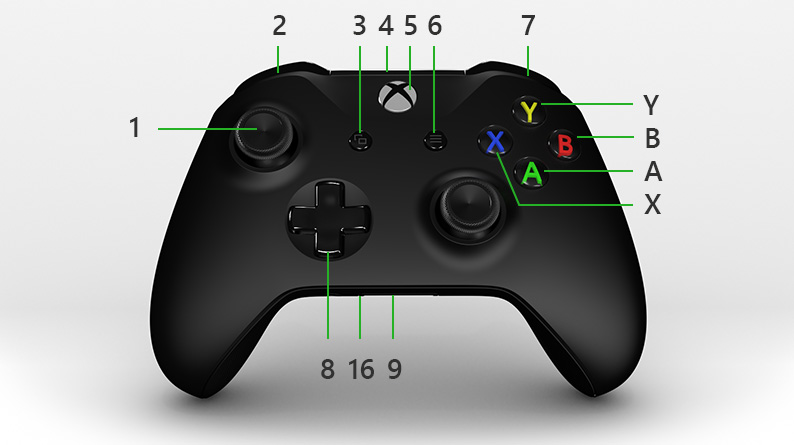
\includegraphics[scale=0.5]{images/vorderseite.jpg}
    \caption{Vorderseite des Controllers}
    \label{fig:vorderseite}
\end{figure}

\begin{figure}[H]
    \centering
    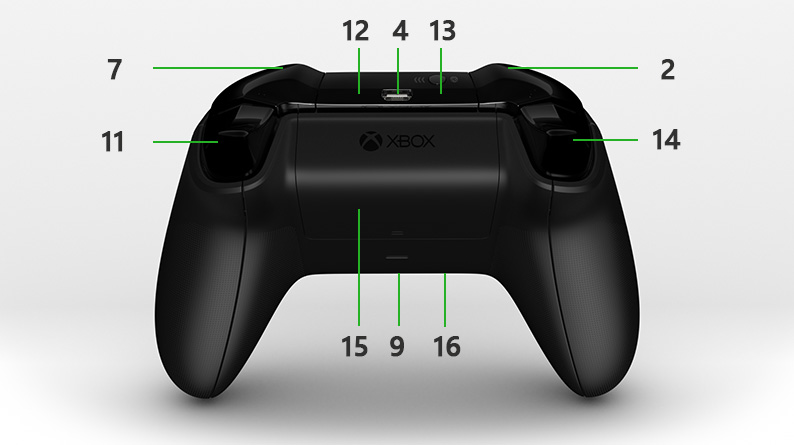
\includegraphics[scale=0.5]{images/rueckseite.jpg}
    \caption{Rückseite des Controllers}
    \label{fig:rueckseite}
\end{figure}

\begin{table}[H]
    \begin{tabular}{|c|c|}
    \hline
    \rowcolor[gray]{0.8}
     Nummerierung der Taste & Funktion \\ \hline 
     1 & Bewegung des Ruders \\ \hline 
     2 & Reduzierung der linken Gashebelposition \\ \hline 
     7 & Reduzierung der rechten Gashebelposition \\ \hline
     11 & Erhöhung der rechten Gashebelposition \\ \hline
     14 & Erhöhung der linken Gashebelposition \\ \hline
     B + 2 + 7 & Einlegen des Rückwärtsgangs \\ \hline
    \end{tabular}
\end{table}

\section{Integration des Rogue Device}
Damit der Controller die Steuerbefehle an das Schiff senden kann, muss das Rogue Device in das System integriert werden.
In diesem Fall ist das Rogue Device der Raspberry Pi. Damit dieser möglichst unbemerkt in das System integriert werden könnte,
muss der Controller drahtlos verbunden werden. Um die Kommunikation von dem Rogue Device zu dem Schiff zu ermöglichen, müssen
die einzelnen Systeme angesteuert werden. Um die Gashebelposition zu verändern, wird der Raspberry Pi mit dem Can-Bus des Schiffes
verbunden. 
\\
Sollte der Gashebel in der normalen Benutzung vom Schiffsführer benutzt werden, wird ein Signal an den Can-Bus gesendet. Dieses Signal wird dann an die Motoren weitergeleitet.
Um diese Eingabe zu verhindern, muss auf diese Nachricht geachtet und reagiert werden. Mit dem Lesen des Can-Bus kann die 
entsprechende Nachricht entdeckt werden. Dann kann eine Nachricht von dem Rogue Device gesendet werden, um die Gashebelposition
zu überschreiben.
\\
Um eine Rückmeldung zu erhalten, wie die gewünschte Gashebel- und Ruderposition ist, sollte mit einer einfachen App
gearbeitet werden. Diese App kann dann die gewünschten Positionen anzeigen. Ein kleiner OLED-Bildschirm könnte auch benutzt 
werden. Allerdings hat dieser den Nachteil, dass er physisch an den Raspberry Pi angeschlossen werden muss. Damit 
ist keine Rückmeldung möglich, wenn dieser als Rogue Device in dem System versteckt angeschlossen ist.
Um die Kommunikation zwischen dem Raspberry Pi und dem Handy mit der App zu ermöglichen, wird Bluetooth benutzt.


\begin{itemize}
    \item Was passiert bei Veränderung der Gashebelposition?
    \item Wie passiert die Rückmeldung
\end{itemize}
Was muss ich dabei beachten?
Muss eine Rückmeldung für die Eingaben geschehen? Wenn ja, wie?
(kleiner OLED-Bildschirm oder App)
